\documentclass[a4paper,12pt]{article}
\usepackage{amsmath, amssymb}
\usepackage{tikz}
\usetikzlibrary{trees}
\usepackage{listings}
\usepackage{xcolor}

\title{3-adischer Steuer-Baum (Blocktree) mit EU-Verteilung}
\author{Alexander Kern}
\date{\today}

\lstset{
  basicstyle=\ttfamily\small,
  keywordstyle=\color{blue}\bfseries,
  commentstyle=\color{green}\itshape,
  stringstyle=\color{red},
  showstringspaces=false
}

\begin{document}
\maketitle

\section{Hierarchie des Baums (Blocktree)}
\begin{center}
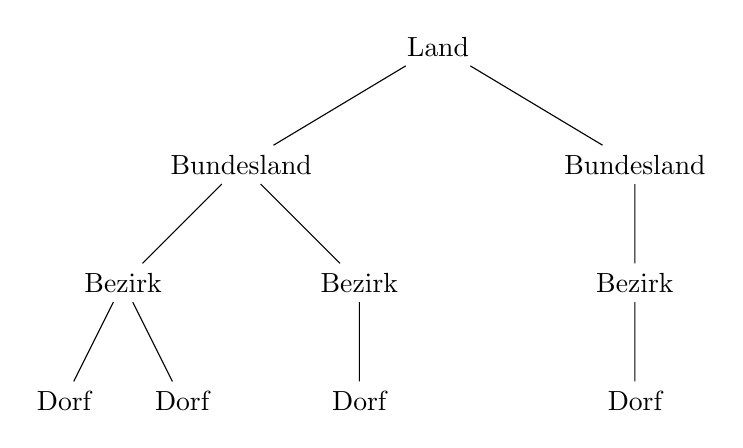
\begin{tikzpicture}[level distance=1.5cm,
  level 1/.style={sibling distance=5cm},
  level 2/.style={sibling distance=3cm},
  level 3/.style={sibling distance=1.5cm}]
\node {Land}
  child {node {Bundesland}
    child {node {Bezirk}
      child {node {Dorf}}
      child {node {Dorf}}
    }
    child {node {Bezirk}
      child {node {Dorf}}
    }
  }
  child {node {Bundesland}
    child {node {Bezirk}
      child {node {Dorf}}
    }
  };
\end{tikzpicture}
\end{center}

\section{Steuern und Zweckbindung}
\begin{align*}
\text{tax}_\text{dorf} &= \text{tax}_\text{infra} + \text{tax}_\text{transfer} \\
\text{tax}_\text{infra} &= p_\text{infra} \cdot \text{tax}_\text{dorf} \\
\text{tax}_\text{transfer} &= (1 - p_\text{infra}) \cdot \text{tax}_\text{dorf} \\
\text{tax}_\text{infra}^{\text{node}} &= \text{tax}_\text{infra}^{\text{local}} + \sum_{c} \text{tax}_\text{infra}^c \\
\text{tax}_\text{transfer}^{\text{node}} &= \text{tax}_\text{transfer}^{\text{local}} + \sum_{c} \text{tax}_\text{transfer}^c
\end{align*}

\section{EU-Verteilung der Transfers}
\[
\text{tax}_\text{EU-Land} = \frac{\text{tax}_\text{transfer}^{\text{Land}}}{n_\text{EU-Länder}}, \quad 1 \le n_\text{EU-Länder} \le 3
\]

\section{Blocktree-Hashes}
Jeder Knoten bekommt einen Hash:
\[
\text{hash}_\text{node} = H\Big(\text{name}_\text{node} \,\|\, \text{parent\_hash} \,\|\, \big\|_{c \in \text{children}} \text{hash}_c \Big)
\]

\section{Pseudocode: Steuern, Transfers und Blocktree}
\begin{verbatim}
Function GenerateNode(level, depth, parentHash):
    Name = generateName(level)
    if level == "Dorf":
        localTax = computeLocalTax()
        taxInfra = pInfra * localTax
        taxTransfer = (1-pInfra) * localTax
    else:
        children = []
        for 1..rand(1,3):
            child = GenerateNode(nextLevel(level), depth-1, parentHash)
            children.append(child)
        taxInfra = sum(child.taxInfra for child in children)
        taxTransfer = sum(child.taxTransfer for child in children)
    hash = SHA256(Name + parentHash + concat(child.hashes))
    return Node(Name, taxInfra, taxTransfer, hash, children)

Function DistributeEU(node, EU_Laender):
    share = node.taxTransfer / len(EU_Laender)
    for each country in EU_Laender:
        country.tax += share
\end{verbatim}

\section{C++ Implementation}
\begin{lstlisting}[language=C++]
#include <iostream>
#include <vector>
#include <string>
struct Node {
    std::string name;
    double localTax = 0.0;
    double taxInfra = 0.0;
    double taxTransfer = 0.0;
    std::string hash;
    std::vector<Node> children;
};

double computeTax(Node& node){
    node.taxInfra = node.localTax*0.6;
    node.taxTransfer = node.localTax*0.4;
    for(auto& c : node.children){
        computeTax(c);
        node.taxInfra += c.taxInfra;
        node.taxTransfer += c.taxTransfer;
    }
    return node.taxInfra + node.taxTransfer;
}

void computeHash(Node& node, const std::string& parentHash=""){
    std::string data = node.name + parentHash;
    for(auto& c : node.children) data += c.hash;
    node.hash = "HASH_PLACEHOLDER";
    for(auto& c : node.children) computeHash(c, node.hash);
}

void distributeEU(Node& node, std::vector<Node>& EU){
    double share = node.taxTransfer / EU.size();
    for(auto& country : EU) country.taxTransfer += share;
}
\end{lstlisting}

\section{Java Implementation}
\begin{lstlisting}[language=Java]
class Node {
    String name;
    double localTax;
    double taxInfra;
    double taxTransfer;
    String hash;
    List<Node> children = new ArrayList<>();

    double computeTax(){
        taxInfra = 0.6*localTax;
        taxTransfer = 0.4*localTax;
        for(Node c : children){
            c.computeTax();
            taxInfra += c.taxInfra;
            taxTransfer += c.taxTransfer;
        }
        return taxInfra + taxTransfer;
    }

    void computeHash(String parentHash){
        String data = name + parentHash;
        for(Node c : children) data += c.hash;
        hash = "HASH_PLACEHOLDER";
        for(Node c : children) c.computeHash(hash);
    }

    void distributeEU(List<Node> EU){
        double share = taxTransfer / EU.size();
        for(Node country : EU) country.taxTransfer += share;
    }
}
\end{lstlisting}

\section{Haskell Implementation}
\begin{lstlisting}[language=Haskell]
data Node = Node {
    name :: String,
    localTax :: Double,
    taxInfra :: Double,
    taxTransfer :: Double,
    hashVal :: String,
    children :: [Node]
} deriving Show

computeTax :: Node -> Node
computeTax n =
    let infra = 0.6 * localTax n
        transfer = 0.4 * localTax n
        updatedChildren = map computeTax (children n)
        totalInfra = infra + sum (map taxInfra updatedChildren)
        totalTransfer = transfer + sum (map taxTransfer updatedChildren)
    in n { taxInfra = totalInfra, taxTransfer = totalTransfer, children = updatedChildren }

computeHash :: Node -> String -> Node
computeHash n parentHash =
    let childHashes = concatMap hashVal (children n)
        h = "HASH_PLACEHOLDER"
        updatedChildren = map (\c -> computeHash c h) (children n)
    in n { hashVal = h, children = updatedChildren }

distributeEU :: Node -> [Node] -> [Node]
distributeEU node eu =
    let share = taxTransfer node / fromIntegral (length eu)
    in map (\c -> c { taxTransfer = taxTransfer c + share }) eu
\end{lstlisting}

\end{document}

